\documentclass[aspectratio=1610]{beamer}
\usepackage[utf8]{inputenc}
\usepackage{ragged2e}
\usepackage{xcolor}
\usepackage[italian]{babel}
\usepackage{tikz}
\usetheme[progressbar=frametitle,titleformat=smallcaps]{metropolis}
\setbeamertemplate{frame numbering}[fraction]
\setbeamercovered{dynamic}
\definecolor{rosso}{RGB}{255, 0, 0}
\definecolor{giallo}{RGB}{254,212,23}
\hypersetup{colorlinks=true,linkcolor=black,urlcolor=rosso}
\setbeamercolor{palette primary}{fg=black, bg=giallo}
\setbeamercolor{background canvas}{bg=white}
\setbeamercolor{normal text}{fg=black}
\setbeamercolor{progress bar}{fg=rosso}
\setbeamercolor{framesubtitle}{fg=rosso}
\setbeamercolor{normal text .dimmed}{fg=giallo}
\setbeamercolor{block title alerted}{fg=rosso, bg=giallo}
\setbeamerfont{caption}{size=\tiny}
\setbeamerfont{caption name}{size=\tiny}
\setlength{\abovecaptionskip}{0pt}
\makeatletter
\metroset{block=fill}
\setlength{\metropolis@progressinheadfoot@linewidth}{1pt} 
\setlength{\metropolis@progressonsectionpage@linewidth}{1pt}
\setlength{\metropolis@titleseparator@linewidth}{1pt}
\makeatother

\title{USO E ABUSO DEI VIDEOGAMES}
\subtitle{il videogioco come forma di aggregazione}
\date{}
\institute{\textit{
        Fonti:
        \begin{itemize}
            \item[-] \href{https://it.wikipedia.org/wiki/Dipendenza_da_videogiochi}{Wikipedia}
            \item[-] \href{https://icd.who.int/en}{World Health Organization ICD}
            \item[-] \href{https://www.nationalgeographic.it/dipendenza-da-videogiochi-come-uscire-dal-tunnel}{National Geographic}
            \item[-] \href{https://www.treccani.it/vocabolario/community/}{Treccani} 
        \end{itemize}
    }
}

\begin{document}

\begin{frame}[plain, noframenumbering]
    \titlepage
\end{frame}

\section{DIPENDENZA}

\begin{frame}{DIPENDENZA DAI VIDEOGAMES}
    \begin{columns}
        \column{\textwidth}
        \begin{figure}
            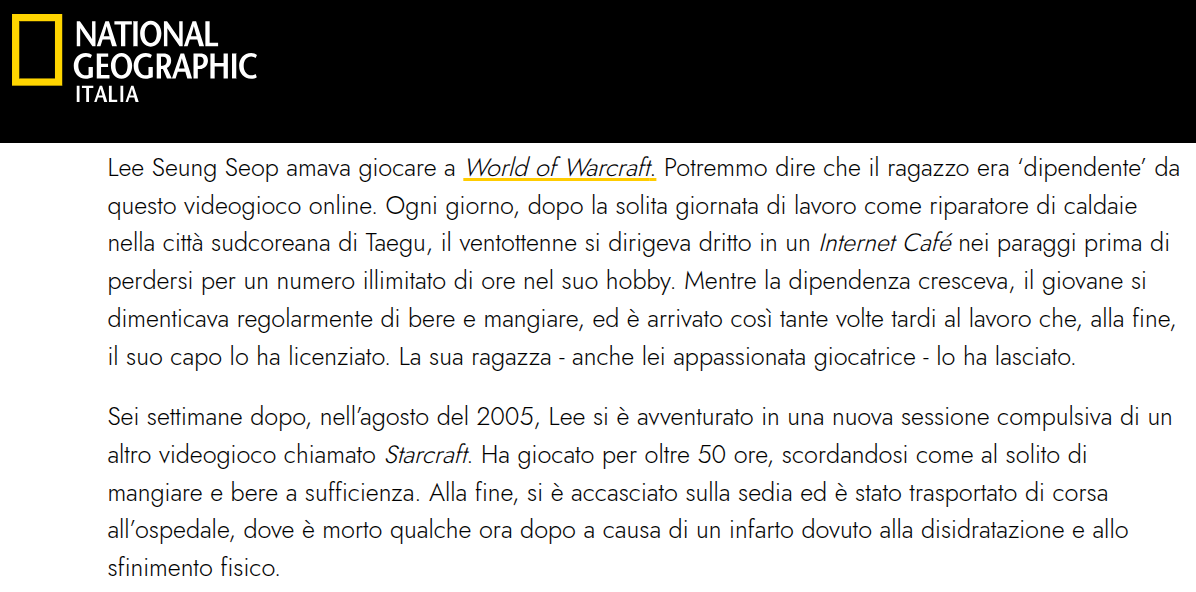
\includegraphics[width=\linewidth]{img/LeeSeungSeop.png}
            \caption{{Fonte \href{https://www.nationalgeographic.it/dipendenza-da-videogiochi-come-uscire-dal-tunnel}{National Geographic}}}
        \end{figure}
    \end{columns}
\end{frame}

\begin{frame}{DIPENDENZA DAI VIDEOGAMES}
    \begin{columns}
        \column{\textwidth}
        \begin{figure}
            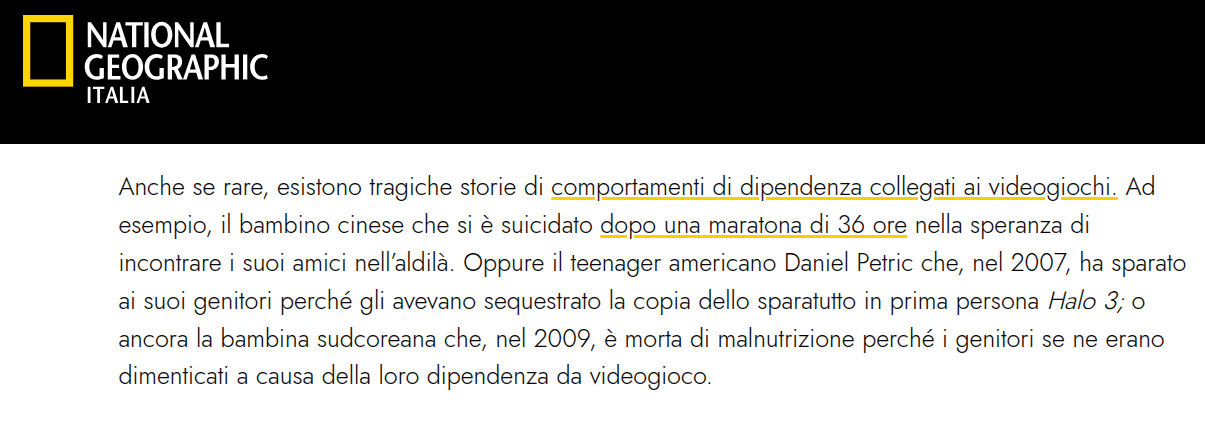
\includegraphics[width=\linewidth]{img/esempi.png}
            \caption{{Fonte \href{https://www.nationalgeographic.it/dipendenza-da-videogiochi-come-uscire-dal-tunnel}{National Geographic}}}
        \end{figure}
    \end{columns}
\end{frame}

\begin{frame}{DIPENDENZA DAI VIDEOGAMES}
    \begin{alertblock}{DEFINIZIONE}
        \begin{minipage}{0.98\linewidth}
            \justifying
            La dipendenza da videogiochi (gaming disorder) è un uso eccessivo o compulsivo di videogiochi, 
            che interferisce con la vita quotidiana di una persona. La dipendenza da videogiochi può presentarsi 
            con una compulsione al gioco, l'isolamento sociale, sbalzi d'umore, ideazione diminuita, 
            e iper-focalizzazione sui risultati del gioco, con esclusione di altri eventi nella vita. 
            È classificata come una dipendenza comportamentale.\\
            \bigskip
            \tiny{\textbf{World Health Organization}}
            \tiny{\href{https://icd.who.int/browse/2025-01/mms/en\#1448597234}{ICD}}
        \end{minipage}
    \end{alertblock}
\end{frame}

\begin{frame}{DIPENDENZA DAI VIDEOGAMES}
    \begin{columns}
        \column{\textwidth}
        \begin{figure}
            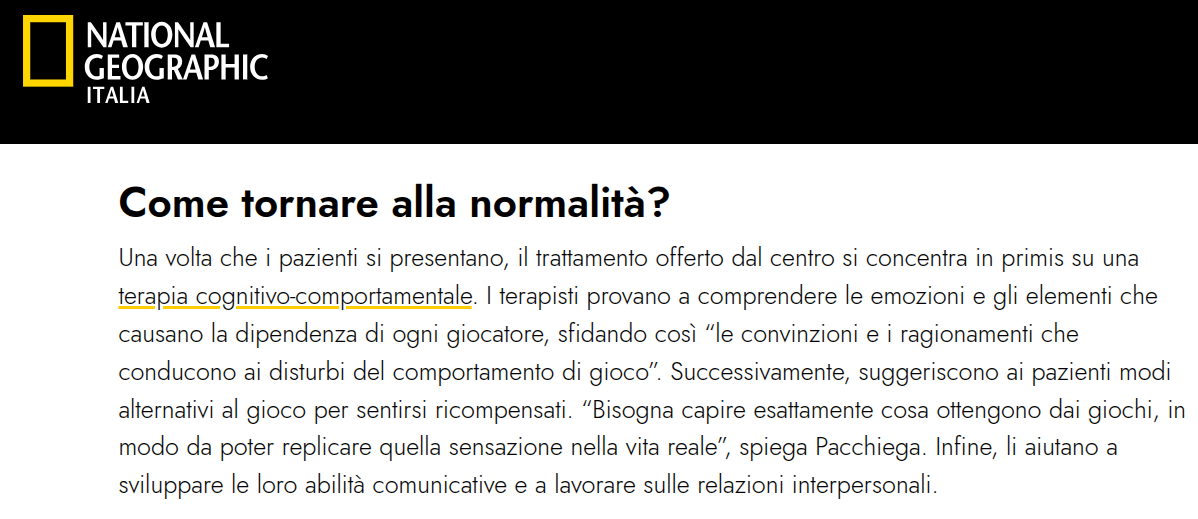
\includegraphics[width=\linewidth]{img/soluzione.png}
            \caption{{Fonte \href{https://www.nationalgeographic.it/dipendenza-da-videogiochi-come-uscire-dal-tunnel}{National Geographic}}}
        \end{figure}
        \begin{tikzpicture}[overlay]
            \draw[red, line width=3pt] (8.1, 1.8) rectangle (11,2.3);
        \end{tikzpicture}
    \end{columns}
\end{frame}

\section{COMMUNITY}

\begin{frame}{COMMUNITY}
    \begin{alertblock}{DEFINIZIONE}
        \begin{minipage}{0.98\linewidth}
            \justifying
            Nel linguaggio di Internet, gruppo di persone che si incontrano, discutono e si scambiano 
            informazioni attraverso la rete (gli strumenti utilizzati più frequentemente dagli utenti per 
            interagire sono forum, chat e programmi di messaggistica istantanea): far parte di una community. 
            Il luogo virtuale in cui avvengono le interazioni tra i membri di una community.\\
            \bigskip
            \tiny{\textbf{Fonte}}
            \tiny{\href{https://www.treccani.it/vocabolario/community/}{Treccani}}
        \end{minipage}
    \end{alertblock}
\end{frame}

\begin{frame}{COMMUNITY}
    \begin{columns}
        \column{.33\textwidth}
        \begin{figure}
            
\includegraphics[width=0.5\linewidth, height=0.5\linewidth]{img/twitch.png}
            \caption{\href{https://www.twitch.tv/}{Twitch}}
        \end{figure}
        \column{.33\textwidth}
        \begin{figure}
            
\includegraphics[width=0.6\linewidth, height=0.5\linewidth]{img/discord.png}
            \caption{\href{https://discord.com/}{Discord}}    
        \end{figure}
        \column{.33\textwidth}
        \begin{figure}
            
\includegraphics[width=0.5\linewidth, height=0.5\linewidth]{img/reddit.png}
            \caption{\href{https://www.reddit.com/}{Reddit}}    
        \end{figure}
    \end{columns}
\end{frame}

\begin{frame}{COMMUNITY}
    \begin{columns}
        \column{\textwidth}
        \begin{figure}
            
\includegraphics[width=\linewidth]{img/isc.png}
            \caption{{\href{https://italianspeedruncommunity.com/}{Italian Speedrun Community}}}
        \end{figure}
    \end{columns}
\end{frame}

\begin{frame}{COMMUNITY}
    \begin{columns}
        \column{\textwidth}
        \begin{figure}
            
\includegraphics[width=\linewidth]{img/warpa.png}
            \caption{{\href{https://zonawarpa.it/}{Zona Warpa}}}
        \end{figure}
    \end{columns}
\end{frame}

\begin{frame}{COMMUNITY}
    \begin{columns}
        \column{\textwidth}
        \begin{figure}
            
\includegraphics[width=\linewidth]{img/mgw.png}
            \caption{\href{https://www.youtube.com/watch?v=OKoTHn0xw3U}{MGW: Milan Games Week}}
        \end{figure}
    \end{columns}
\end{frame}

\end{document}